% ---------------------------------------------------------------------------------------------------------------
% TEMPLATE PARA TRABALHO DE CONCLUSÃO DE CURSO
% Universidade Tecnológica Federal do Paraná - UTFPR
% Customização da classe abnTeX2 (http://www.abntex.net.br/) para as normas da UTFPR
%
% Projeto hospedado em: <link git>
% Autores: Diego Marczal  <>
% 	   Michael Vornes <https://github.com/mvornes>
%
%----------------------------------------------------------------------------------------------------------------
% Codificação: UTF-8
% LaTeX:  abnTeX2          
% ---------------------------------------------------------------------------------------------------------------


% CARREGA CLASSE PERSONALIZADA DA UTFPR--------------------------------------------------------------------------
\documentclass[%twoside,                   % Impressão em frente e verso
    	        oneside,                   % Impressão apenas frente
]{configuracoes/utfpr-abntex2}

% INCLUI ARQUIVOS DE CONFIGURAÇÕES-------------------------------------------------------------------------------
% REFERÊNCIAS------------------------------------------------------------------
\usepackage[%
    alf,
    abnt-emphasize=bf,
    bibjustif,
    recuo=0cm,
    abnt-url-package=url,       % Utiliza o pacote url
    abnt-refinfo=yes,           % Utiliza o estilo bibliográfico abnt-refinfo
    abnt-etal-cite=3,
    abnt-etal-list=3,
    abnt-thesis-year=final
]{abntex2cite}                  % Configura as citações bibliográficas conforme a norma ABNT

% PACOTES----------------------------------------------------------------------
\usepackage[utf8]{inputenc}                                 % Codificação do documento
\usepackage[T1]{fontenc}                                    % Seleção de código de fonte
\usepackage{booktabs}                                       % Réguas horizontais em tabelas
\usepackage{color, colortbl}                                % Controle das cores
\usepackage{float}                                          % Necessário para tabelas/figuras em ambiente multi-colunas
\usepackage{graphicx}                                       % Inclusão de gráficos e figuras
\usepackage{icomma}                                         % Uso de vírgulas em expressões matemáticas
\usepackage{indentfirst}                                    % Indenta o primeiro parágrafo de cada seção
\usepackage{microtype}                                      % Melhora a justificação do documento
\usepackage{multirow, array}                                % Permite tabelas com múltiplas linhas e colunas
\usepackage{subeqnarray}                                    % Permite subnumeração de equações
\usepackage{lastpage}                                       % Para encontrar última página do documento
\usepackage{verbatim}                                       % Permite apresentar texto tal como escrito no documento, ainda que sejam comandos Latex
\usepackage{amsfonts, amssymb, amsmath}                     % Fontes e símbolos matemáticos
\usepackage[algoruled, portuguese]{algorithm2e}             % Permite escrever algoritmos em português
%\usepackage[scaled]{helvet}                                % Usa a fonte Helvetica
\usepackage{times}                                          % Usa a fonte Times
%\usepackage{palatino}                                      % Usa a fonte Palatino
%\usepackage{lmodern}                                       % Usa a fonte Latin Modern
\usepackage[bottom]{footmisc}                               % Mantém as notas de rodapé sempre na mesma posição
\usepackage{ae, aecompl}                                    % Fontes de alta qualidade
\usepackage{latexsym}                                       % Símbolos matemáticos
\usepackage{lscape}                                         % Permite páginas em modo "paisagem"
%\usepackage{picinpar}                                      % Dispor imagens em parágrafos
%\usepackage{scalefnt}                                      % Permite redimensionar tamanho da fonte
%\usepackage{subfig}                                        % Posicionamento de figuras
%\usepackage{upgreek}                                       % Fonte letras gregas

% Redefine a fonte para uma fonte similar a Arial (fonte Helvetica)
\renewcommand*\familydefault{\sfdefault}

% CONFIGURAÇÕES DE APARÊNCIA DO PDF FINAL--------------------------------------
\makeatletter
\hypersetup{%
    portuguese,
    colorlinks=true,   % true: "links" coloridos; false: "links" em caixas de texto
    linkcolor=blue,    % Define cor dos "links" internos
    citecolor=blue,    % Define cor dos "links" para as referências bibliográficas
    filecolor=blue,    % Define cor dos "links" para arquivos
    urlcolor=blue,     % Define a cor dos "hiperlinks"
    breaklinks=true,
    pdftitle={\@title},
    pdfauthor={\@author},
    pdfkeywords={abnt, latex, abntex, abntex2}
}
\makeatother

% ALTERA O ASPECTO DA COR AZUL--------------------------------------------------
\definecolor{blue}{RGB}{41,5,195}

% REDEFINIÇÃO DE LABELS---------------------------------------------------------
\renewcommand{\algorithmautorefname}{Algoritmo}
\def\equationautorefname~#1\null{Equa\c c\~ao~(#1)\null}

% CRIA ÍNDICE REMISSIVO---------------------------------------------------------
\makeindex

% HIFENIZAÇÃO DE PALAVRAS QUE NÃO ESTÃO NO DICIONÁRIO---------------------------
\hyphenation{%
    qua-dros-cha-ve
    Kat-sa-gge-los
}



% INCLUI ARQUIVOS DO TRABALHO DE CONCLUSÃO DE CURSO (PRÉ-TEXTUAIS, TEXTUAIS, PÓS-TEXTUAIS)-----------------------

% INSERE CAPA E FOLHA DE ROSTO


% CAPA---------------------------------------------------------------------------------------------------

% ORIENTAÇÕES GERAIS-------------------------------------------------------------------------------------
% Caso algum dos campos não se aplique ao seu trabalho, como por exemplo,
% se não houve coorientador, apenas deixe vazio.
% Exemplos: 
% \coorientador{}
% \departamento{}

% DADOS DO TRABALHO--------------------------------------------------------------------------------------
\titulo{Classificação de imagem de comida com redes neurais convolucionais}
\titleabstract{Food image classification with convolutional neural networks}
\autor{Rafael Biazus Mangolin}
\autorcitacao{MANGOLIN, Rafael} % Sobrenome em maiúsculo
\local{Maringá}
\data{2017}

% NATUREZA DO TRABALHO-----------------------------------------------------------------------------------
% Opções: 
% - Trabalho de Conclusão de Curso (se for Graduação)
% - Dissertação (se for Mestrado)
% - Tese (se for Doutorado)
% - Projeto de Qualificação (se for Mestrado ou Doutorado)
\projeto{Trabalho de Conclusão de Curso}

% TÍTULO ACADÊMICO---------------------------------------------------------------------------------------
% Opções:
% - Bacharel ou Tecnólogo (Se a natureza for Trabalho de Conclusão de Curso)
% - Mestre (Se a natureza for Dissertação)
% - Doutor (Se a natureza for Tese)
% - Mestre ou Doutor (Se a natureza for Projeto de Qualificação)
\tituloAcademico{Bacharel em Informática}

% ÁREA DE CONCENTRAÇÃO E LINHA DE PESQUISA---------------------------------------------------------------
% Se a natureza for Trabalho de Conclusão de Curso, deixe ambos os campos vazios
% Se for programa de Pós-graduação, indique a área de concentração e a linha de pesquisa
\areaconcentracao{}
\linhapesquisa{}

% DADOS DA INSTITUIÇÃO-----------------------------------------------------------------------------------
% Se a natureza for Trabalho de Conclusão de Curso, coloque o nome do curso de graduação em "programa"
% Formato para o logo da Instituição: \logoinstituicao{<escala>}{<caminho/nome do arquivo>}
\instituicao{Universidade Estadual de Maringá}
\departamento{Departamento de Informática}
\programa{curso de Informática}
% \logoinstituicao{0.2}{dados/figuras/logo-instituicao.png} 

% DADOS DOS ORIENTADORES---------------------------------------------------------------------------------
\orientador{Yandre Maldonado e Gomes da Costa}
%\orientador[Orientadora:]{Nome da orientadora}
\instOrientador{Universidade Estadual de Maringá}

% \coorientador{Nome do coorientador}
%\coorientador[Coorientadora:]{Nome da coorientadora}
% \instCoorientador{Instituição do coorientador}

% FOLHA DE ROSTO--------------------------------------------------------------------------------------------------------

% TRABALHO DE CONCLUSÃO DE CURSO
 \preambulo{{\imprimirprojeto} apresentado ao Curso de Informática, do Centro de Tecnologia, da Universidade Estadual de Maringá.}

% DISSERTAÇÃO DE MESTRADO
% \preambulo{{\imprimirprojeto} apresentada ao Programa de \mbox{Pós-graduação} da {\imprimirinstituicao}, como requisito parcial para obtenção do título de {\imprimirtituloAcademico}.}

% TESE DE DOUTORADO
% \preambulo{{\imprimirprojeto} apresentada ao Programa de \mbox{Pós-graduação} da {\imprimirinstituicao}, como requisito parcial para a obtenção do título de {\imprimirtituloAcademico}.}

% PROJETO DE QUALIFICAÇÃO DE MESTRADO OU DOUTORADO
%\preambulo{{\imprimirprojeto} apresentado ao Programa de \mbox{Pós-graduação} da {\imprimirinstituicao}, como requisito parcial para a obtenção do título de {\imprimirtituloAcademico}.}

% OBSERVAÇÕES-----------------------------------------------------------------------------------------------------------
% Altere este arquivo APENAS comentando as linhas que não se aplicam ao tipo de trabalho acadêmico desejado.



\begin{document}

\pretextual
\imprimircapa                                               	           % Comando para imprimir Capa
\imprimirfolhaderosto{}                                     		   % Comando para imprimir Folha de rosto
% INSERE ELEMENTOS PRÉ-TEXTUAIS
% % DEDICATÓRIA------------------------------------------------------------------

\renewcommand{\dedicatorianame}{DEDICATÓRIA}

\begin{dedicatoria}

Altere este texto inserindo a dedicatória do seu trabalho. 

\end{dedicatoria}
          			   % Dedicatória
% AGRADECIMENTOS---------------------------------------------------------------

\begin{agradecimentos}[AGRADECIMENTOS]

A minha família pelo incentivo e apoio incondicional.
\par Aos meus amigos de graduação, pelas trocas de ideias, críticas e auxílios.
\par Ao meu orientador Dr. Yandre Maldonado e Gomes da Costa, por me apresentar a área de sistemas inteligentes, pelo auxílio e sugestões no desenvolvimento deste trabalho.
\par A todos que direta ou indiretamente fizeram parte da minha formação. 
\end{agradecimentos}
        			   % Agradecimentos
% % EPÍGRAFE---------------------------------------------------------------------

\renewcommand{\epigraphname}{EPÍGRAFE}

\begin{epigrafe}

\textit{Eu denomino meu campo de Gestão do Conhecimento, mas você não pode gerenciar conhecimento. Ninguém pode. O que pode fazer - o que a empresa pode fazer - é gerenciar o ambiente que otimize o conhecimento. (PRUSAK, Laurence, 1997).}

\end{epigrafe}

% OBSERVAÇÕES------------------------------------------------------------------
% Altere o texto para inserir a epígrafe do seu trabalho

              			   % Epígrafe
% RESUMO--------------------------------------------------------------------------------

\begin{resumo}[RESUMO]
\begin{SingleSpacing}

% Não altere esta seção do texto--------------------------------------------------------
\imprimirautorcitacao. \imprimirtitulo. \imprimirdata. \pageref {LastPage} f. \imprimirprojeto\ – \imprimirprograma, \imprimirinstituicao. \imprimirlocal, \imprimirdata.\\
%---------------------------------------------------------------------------------------


Esta monografia aborda o problema de classificação de imagens de comida, que está inserido na área de reconhecimento de padrões. A tarefa de classificação de imagens foi realizada neste trabalho utilizando redes neurais convolucionais (\textit{convolutional neural networks}, CNN), uma técnica de \textit{deep learning}. A CNN é uma rede neural de muitas camadas na qual é aplicada a operação de convolução. A utilização de CNN vem melhorando o estado da arte na área de classificação de imagens desde 2012. Um dos maiores problemas encontrados para o uso de CNN em tarefas de classificação é o \textit{overfitting}, que ocorre devido a uma quantidade escassa de amostras ou dada a profundidade da rede criada. Para a solução desse problema, neste trabalho, foi realizado o \textit{fine tunning} na taxa de \textit{dropout} e foram utilizadas duas técnicas: o \textit{data augmentation} e a inicialização dos pesos da rede a partir de uma rede treinada. A rede neural proposta neste projeto tem como base a CNN \textit{AlexNet}. A base de dados utilizada foi formulada com amostras retiradas das bases \textit{ImageNet} e \textit{Food-101}, contendo 16 classes de imagens. O melhor resultado foi obtido quando aplicada as técnicas de \textit{data augmentation}, \textit{dropout} e inicialização dos pesos, resultando em uma acurácia de 74,56\%.



% Rede neural convolucional (\textit{convolutional neural network}, CNN) foi utilizada neste trabalho para realizar a tarefa de classificação. As CNNs são técnicas de \textit{deep leaning}, que utilizam por meio de redes neurais de muitas camadas para realizar os processos de aprendizado e classificação e vem melhorando o estado da arte na área de classificação de imagens desde 2012. O \textit{overfitting} é um problema recorrente em classificadores que utilizam CNN, esse problema ocorre geralmente devido a falta de amostras para a realização do treino da rede neural. Para a solução desse problema neste trabalho foi proposto duas técnicas: o \textit{data augmentation} e a inicialização dos pesos da rede a partir de uma rede treinada. A rede neural proposta neste projeto tem como base de estrutura a CNN \textit{AlexNet}. A base de dados utilizada foi formulada com amostras retiradas das bases \textit{ImageNet} e \textit{Food-101}, contendo 16 classes de imagens. O melhor resultado foi obtido quando aplicada as técnicas propostas, resultando em uma acurácia de 74,56\%.

\textbf{Palavras-chave}: Classificação de imagens. Rede neural convolucional. \textit{Deep learing}.

\end{SingleSpacing}
\end{resumo}

% OBSERVAÇÕES---------------------------------------------------------------------------
% Altere o texto inserindo o Resumo do seu trabalho.
% Escolha de 3 a 5 palavras ou termos que descrevam bem o seu trabalho 

             			   % Resumo em Português
% ABSTRACT--------------------------------------------------------------------------------

\begin{resumo}[ABSTRACT]
\begin{SingleSpacing}

% Não altere esta seção do texto--------------------------------------------------------
\imprimirautorcitacao. \imprimirtitleabstract. \imprimirdata. \pageref {LastPage} f. \imprimirprojeto\ – \imprimirprograma, \imprimirinstituicao. \imprimirlocal, \imprimirdata.\\
%---------------------------------------------------------------------------------------

This monograph approaches the problem of food image classification, which is inserted in the area of pattern recognition. Convolutional neural network (CNN), was used to perform the classification task. The CNNs has been improving the state of the art in the area of image classification since 2012. CNNs are deep learing techniques, that use through multi-layers neural networks to accomplish the processes of learning and classification. CNNs present a recurring problem in the classification process, the overfitting, this problem usually occurs due to the lack of samples for performing neural network training. To solve this problem in this work two techniques have been proposed: the data augmentation and the initialization of network weights from a trained network. The proposed neural network in this project is based on CNN AlexNet. The database used was formulated with samples taken from the bases ImageNet and Food-101, containing 16 classes of images. The best result was obtained when applying the proposed techniques.

\textbf{Keywords}: Food image classification. Convolutional neural network. Deep learing.

\end{SingleSpacing}
\end{resumo}

% OBSERVAÇÕES---------------------------------------------------------------------------
% Altere o texto inserindo o Abstract do seu trabalho.
% Escolha de 3 a 5 palavras ou termos que descrevam bem o seu trabalho 
             		           % Resumo em Inglês
% Lista de Figuras----------------------------------------------------------------

\pdfbookmark[0]{\listfigurename}{lof}
\listoffigures*
\cleardoublepage

% OBSERVAÇÕES---------------------------------------------------------------------
% Este arquivo não precisa de ser alterado, pois a lista é gerada automaticamente.
   % Lista de Figuras
% % LISTA DE QUADROS----------------------------------------------------------------

\renewcommand{\listofquadrosname}{LISTA DE QUADROS}

\pdfbookmark[0]{\listofquadrosname}{loq}
\listofquadros*
\cleardoublepage

% OBSERVAÇÕES---------------------------------------------------------------------
% Este arquivo não necessita de ser editado. A lista é gerada automaticamente.
   % Lista de Quadros
% LISTA DE TABELAS-------------------------------------------------------------

\pdfbookmark[0]{\listtablename}{lot}
\listoftables*
\cleardoublepage

% OBSERVAÇÕES-------------------------------------------------------------------
% Este arquivo não precisa ser alterado, pois a lista é gerada automaticamente.
         		   % Lista de Tabelas
% % LISTA DE ABREVIATURAS E SIGLAS----------------------------------------------------------

\begin{siglas}
    \item[ABNT] Associação Brasileira de Normas Técnicas
    \item[DECOM] Departamento de Computação
\end{siglas}

% OBSERVAÇÕES-----------------------------------------------------------------------------
% Altere a lista acima para definir os acrônimos e siglas utilizados neste trabalho
          		   % Lista de Abreviaturas e Siglas
% % LISTA DE SÍMBOLOS------------------------------------------------------------

\begin{simbolos}
    \item[$ \Gamma $] Letra grega Gama
    \item[$ \lambda $] Comprimento de onda
    \item[$ \in $] Pertence
\end{simbolos}

% OBSERVAÇÕES-------------------------------------------------------------------
% Altere a lista acima para definir os símbolos utilizados no trabalho
        		   % Lista de Símbolos
% % LISTA DE ALGORITMOS----------------------------------------------------------

\newcommand{\algoritmoname}{Algoritmo}
\renewcommand{\listalgorithmcfname}{LISTA DE ALGORITMOS}

\floatname{algocf}{\algoritmoname}
\newlistof{listofalgoritmos}{loa}{\listalgoritmoname}
\newlistentry{algocf}{loa}{0}

\counterwithout{algocf}{chapter}
\renewcommand{\cftalgocfname}{\algoritmoname\space}
\renewcommand*{\cftalgocfaftersnum}{\hfill--\hfill}

\pdfbookmark[0]{\listalgorithmcfname}{loa}
\listofalgorithms
\cleardoublepage

% OBSERVAÇÕES------------------------------------------------------------------
% Este arquivo não precisa ser alterado, pois a lista é gerada automaticamente.
   % Lista de Algoritmos
% SUMÁRIO----------------------------------------------------------------------

\renewcommand{\contentsname}{SUMÁRIO}

\pdfbookmark[0]{\contentsname}{toc}
\tableofcontents*
\cleardoublepage

% OBSERVAÇÕES-------------------------------------------------------------------
% Este arquivo não precisa ser alterado, pois o sumário é gerado automaticamente.
               			   % Sumário

\textual
% % INSERE ELEMENTOS TEXTUAIS
% INTRODUÇÃO-------------------------------------------------------------------

\chapter{INTRODUÇÃO}
\label{chap:introducao}
O problema de classificação de imagens utilizando técnicas tradicionais de aprendizado de máquina requer conhecimento e experiência no domínio que será classificado, para extrair características (do inglês \textit{features}) relevantes, que são utilizadas para a obter a classificação. Assim, utilizando técnicas que não dependem de extratores especializados de \textit{features}, como redes neurais convolucionais (CNN, \textit{convolutional neural networks}), se torna mais fácil desenvolver modelos eficazes de aprendizado de máquina para novos conjuntos de dados. Nesse projeto foi utilizada CNN para a classificação de imagens com comida, assim não será preciso encontrar descritores especializados nesse domínio. 
\par Segundo \citeonline{lecun2015deep}, o \textit{deep learning} vem sendo utilizado para resolver problemas computacionalmente complexos que temos no nosso dia-a-dia, e seu uso vem evoluindo o estado-da-arte de muitas áreas.
\par Um dos grandes problemas encontrados no uso de CNN é o \textit{overfitting} \cite{imaginetArticle} que ocorre devido a muitos parâmetros na rede ou uma base de dados pequena. A utilização de técnicas como o \textit{dropout} e o \textit{data augmentation} vem sendo utilizas para reduzir o \textit{overfitting} \cite{srivastava2014dropout}.

\par Neste projeto utilizamos de \textit{deep learning}, mais especificamente, de rede neural convolucional, para fazer o reconhecimento e classificação de imagens de comida, visando reconhecer o tipo de comida descrito na imagem, a partir de um conjunto de tipos previamente definidos. Foi aplicada na arquitetura da rede a operação de \textit{dropout} e a técnica de \textit{data augmentation} na base de dados visando reduzir o \textit{overfitting}. 
\par Na \autoref{chap:fundamentacaoTeorica} de revisão de literatura desse projeto são descritos conceitos que auxiliam no seu desenvolvimento, sendo dividida em dois tópicos principais: Redes Neurais e \textit{Deep learning}. A \autoref{chap:metodologia} de metodologia descreve como foi estruturado o projeto, e as etapas utilizadas na sua aplicação, é composta por três tópicos principais: a definição e organização da base de dados; a arquitetura da rede neural proposta; e técnicas para melhorar o poder de classificação da rede neural.
\par A \autoref{chap:resultados} de resultados apresenta os valores obtidos com os experimentos realizados, contendo uma comparação entre os resultados e avaliando as melhorias obtidas conforme as técnicas eram adicionadas ao modelo. A melhora na acurácia e a redução do \textit{overfitting} são pontos discutidos. Na \autoref{chap:conclusao} de conclusão é apresentada uma síntese sobre o modelo e os resultados obtidos, também é proposta situações para a continuação deste trabalho.
                		           % Introdução
% REVISÃO DE LITERATURA--------------------------------------------------------

\chapter{REVISÃO DE LITERATURA}
\label{chap:fundamentacaoTeorica}

Nesta seção, será descrita a revisão de literatura sobre redes neurais, \textit{deep learning} e redes neurais convolucionais.

\section{Rede neural}
Rede neural artificial pode ser definida como sendo um conjunto interconectado de elementos básicos de processamento \cite{Gurney1997}. Seu funcionamento é inspirado na capacidade de aprendizado do cérebro animal, que possui uma imensa estrutura com capacidade de definir regras a partir de experiências, que vão ocorrendo durante a vida, gerando ligações físicas (sinapses) mais fortes, aprimorando assim o que foi aprendido \cite{haykin2001}.
\begin{citacao}
  Uma rede neural é um processador maciçamente paralelo e distribuído, constituído de unidades de processamento simples, que tem a propensão natural para armazenar conhecimento experimental e torna-ló disponível para uso. Ela se assemelha ao cérebro em dois aspectos: o conhecimento é adquirido pela rede a partir de seu ambiente por meio de um processo de aprendizagem; forças de conexão entre neurônios, definidos como pesos sinápticos, são utilizados para armazenar o conhecimento adquirido \cite{haykin2001}.
\end{citacao}

\par Dadas essas características, as redes neurais vem sendo amplamente utilizadas para resolução de problemas que não possuem uma resolução trivial, como a classificação de imagens \cite{imaginetArticle}, a identificação de câncer de pele \cite{esteva2017dermatologist}, tomada de decisão no mercado de ações \cite{gambogi2013aplicaccao}, e entre outras áreas. Essa versatilidade de áreas em que é utilizada ocorre devido a sua generalidade na maneira de encontrar pontos no problema que devem ter mais destaque, características mais relevantes que são identificada pela rede durante seu processo de aprendizagem, sendo reavaliadas pela própria rede em cada instância testada. Como dito por \citeonline{zhang2000neural}, as redes neurais possuem a habilidade de se adaptar aos dados para realizar as classificações sem a necessidade de apontar explicitamente o que deve ser observado no modelo.
\par Segundo \citeonline{Kriesel2007NeuralNetworks} uma rede neural pode ser descrita por três elementos:
\begin{itemize}
\item Unidades simples de processamento, ou neurônios.
\item Elos de conexão entre os neurônios (sinapses).
\item A importância entre a conexão de um neurônio com outro, descrita por uma função de peso \textit{w}.
\end{itemize}
\par Uma rede neural pode ser descrita matematicamente pela tríplice ($N$,$V$,$w$), onde $N$ é um conjunto de neurônios, $V$ é um conjunto de conexões entre os neurônios definida por $V = \{($i,$j) \,|\, $i,$j \in N \}$ e $w$ é a função que determina o peso das conexões definida por $w: V \implies \mathbb{R}$, descrita em $w(i,j)$.
\subsection{Neurônio}
\citeonline{haykin2001} define o neurônio como a unidade de processamento de informação que é primordial para o funcionamento de uma rede neural artificial. É nele que ocorre o processamento das entradas, e o redirecionamento da saída, indicando onde irá influenciar tal processamento.
\par Na \autoref{fig:neuronio} é possível identificar os três elementos fundamentais de um neurônio:

\begin{figure}[H]
  \centering
  \caption{Modelo de um neurônio, contendo as entradas, funções de peso, função somadora, o \textit{bias}, função de ativação da saída.}
  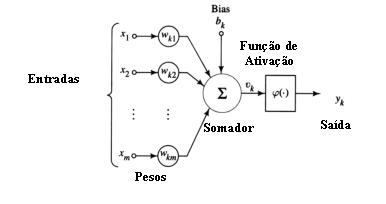
\includegraphics[width=300pt]{dados/figuras/neuron}
  \fonte{imagem retirada do \textit{Google}\protect\footnotemark}
  \label{fig:neuronio}
\end{figure}

\footnotetext{http://www.gsigma.ufsc.br/popov/aulas/rna/neuronio\_artificial/neuronio\_artificial.jpg, acessada em 02 de junho de 2017, ás 18:53}
\begin{itemize}
\item O fluxo de entrada dos dados, sendo ele um conjunto de conexões que serão sujeitas a função de peso, para ser feito o uso na função somadora \cite{haykin2001}. As conexões podem se originar tanto de uma entrada de dados na rede, quanto de neurônios que estão localizados em camadas superiores.
\item A função somadora é responsável por realizar o processamento do fluxo de entrada.
Um exemplo desse tipo de função é a soma dos pesos \cite{Kriesel2007NeuralNetworks}, a função realiza a multiplicação do peso $w_{kj}$ com a entrada $x_j$, e depois realiza a soma das $m$ entradas do neurônio representada pela função matemática:
\par \[u_k = sum_{j=1}^{m} w_{kj}x_j\]
\par O resultado dessa etapa é propagado pela rede dados os critérios da função de ativação.
\item A função de ativação é responsável por restringir a abrangência do dado gerado pelo processamento do neurônio. Foi identificado por \citeonline{haykin2001} três tipos básicos de função de ativação sendo elas:
  \begin{itemize}
    \item \textbf{Função de limiar}:
\[ f(x)= \begin{cases} 1&se \ x \ge 0 \\ -1 & se\ x < 0 \end{cases} \]
      \par É conhecido na literatura como função de \textit{Heaviside}, definindo a saída de maneira binaria.
    \item \textbf{Função linear por partes}: 
\[ f(x)= \begin{cases} 1&se \ x \ge 1 \\x & se\ 0\le x < 1 \\ 0 & se\ x < 0 \end{cases} \]
      \par Esse tipo de função pode ser analisada como uma tentativa de simulação de um amplificador não linear, tendo sua área variável e seus pontos de saturação. 
    \item \textbf{Função Sigmoide}: 
\[ f(x)= \frac{1}{1 + exp(-av)} \]
      \par Esse tipo de função de ativação é o mais utilizado na construção de redes neurais artificiais \cite{haykin2001}. É definida por uma função crescente não linear, quando seu parâmetro de curva se aproxima do infinito, apresenta comportamento semelhante a funções de limiar.
  \end{itemize}
\end{itemize}
\par O modelo neural da figura acima também inclui um \textit{bias} $(b_k)$ aplicado externamente. Tem como função aumentar ou diminuir a entrada mínima de dados. Defini um limiar no neurônio e pode ser utilizado para o cálculo da função de ativação. 
\par Dado as iteração, a \textit{bias} e os pesos da entrada podem ser modificados pelo processo de aprendizagem, aprimorando sua resposta conforme a rede é treinada.  
\subsection{Processos de aprendizagem}
A habilidade que se destaca de uma rede neural é a aprendizagem, adaptando-se aos dados que estão em seu ambiente, para melhorar o seu desempenho. Essa habilidade vem do processo de aprendizagem da rede neural artificial, que é definido por \citeonline{Demuth:2014:NND:2721661} como o procedimento de ajuste das funções de pesos e dos \textit{bias} dos neurônios da rede, acontecendo na etapa de \textit{"treino"} da rede e tem como objetivo preparar a rede para executar uma tarefa. 
\par Podemos dividir o processo de aprendizagem em três categorias principais sendo elas:
\begin{itemize}
\item \textbf{Aprendizado supervisionado:} método no qual uma parte da base é utilizada para treinar a rede. Assim após cada processamento é verificado o resultado da classificação, e se necessário são feitas correções nos pesos dos neurônios que influenciaram esse resultado, para assim reforçar uma classificação boa ou corrigir uma classificação ruim.
\item \textbf{Aprendizado por reforço:} método similar ao aprendizado supervisionado, tendo como diferença a forma de avaliação. Como dito por \citeonline{kaelbling1996reinforcement}, a principal diferença entre aprendizagem supervisionada e a aprendizagem por reforço, é que o aprendizado por reforço não apresenta conjuntos de saídas corretos e errados, e após cada ação é aplicado uma taxa de correção e indicado os estados seguintes, mas não é informado qual escolha teria sido a melhor para o caso.
\item \textbf{Aprendizado não-supervisionado:} método no qual não existe um avaliador ou dados pré-definido informando a classe da entrada, a própria rede é responsável por agrupar os dados, os ajustes dos pesos e dos \textit{bias} é feito apartir das entradas. A rede basicamente aprende como categorizar a entrada de dados em uma quantidade finita de classes. 
\end{itemize}	
\subsection{\textit{Perceptron}}
O \textit{perceptron} é tido como a forma mais simples de rede neural para classificar duas classes que são linearmente separáveis \cite{haykin2001}. Como essa rede é composta por um único neurônio com pesos de conexões e \textit{bias} ajustáveis está limitado a classificar a entrada apenas em duas classes. 
\par A rede é inicializada com pesos aleatórios, e após a execução de cada entrada sua saída é comparada com o resultado esperado, obtendo assim um sinal de erro, que é utilizado para fazer ajustes nos pesos. Como ocorre nos processos de aprendizado supervisionado.
\par Uma generalização do \textit{perceptron}, é o perceptron de múltiplas camadas (no inglês \textit{multiple layer perceptron}, MLP). Onde o MLP é configurado em no mínimo três camadas, onde a primeira delas é a camada de entrada, em que ocorrem a entrada dos dados na rede, e a última é a camada de saída onde está contida a classificação da entrada. As camadas intermediárias tem a função de analisar características mais complexas da entrada, dando possibilidade de uma melhor classificação.
\par O método de aprendizagem utilizado pelo \textit{perceptron} de múltiplas camadas é conhecido como \textit{error backpropagation} (algorítimo de retropropagação de erro) \cite{haykin2001}. Para isso, utiliza do método de aprendizado supervisionado de correção por erro. Quando é identificada a necessidade de ajuste nos pesos, ocorre uma 
retropropagação nos neurônios que influenciaram a classificação, ajustando seus pesos 
e \textit{bias}.
\subsection{Tipos de redes}
Para problemas mais complexos, redes com apenas um neurônio tendem a não resolve-los. Geralmente é necessário ter vários deles trabalhando em paralelo (uma camada de neurônios) \cite{Demuth:2014:NND:2721661}. \cite{haykin2001} descreve três classes de arquitetura de rede que geralmente são encontradas:
\begin{itemize}
\item \textbf{Redes alimentadas adiante de uma camada:} essa classe é a forma mais simples de rede em camada, na qual se tem uma camada de dados e uma camada de neurônios (camada de processamento), que também é a camada de saída, como na \autoref{fig:umacamada}. A camada de entrada de dados não é contada, pois nela não ocorre processamento.
\begin{figure}[H]
  \centering
  \caption{Exemplo de rede alimentada adiante de uma camada.}
  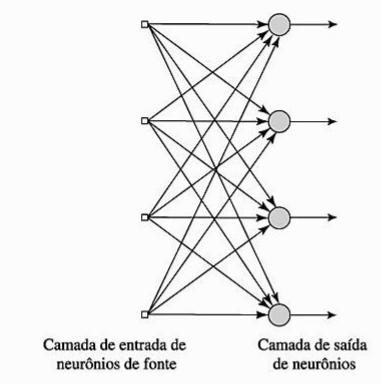
\includegraphics[width=180pt]{dados/figuras/uma_camada}
  \fonte{\cite{haykin2001}}
  \label{fig:umacamada}
\end{figure}

\item \textbf{Redes alimentadas diretamente com múltiplas camadas:} essa classe de rede, é também alimentada adiante, mas possui uma ou mais camadas ocultas. As camadas ocultas estão localizadas entre a camada de entrada de dados e a camada de saída. Ao adicionar camadas ocultas na rede é  possível ter acesso a características mais específicas da entrada, melhorando o resultado da rede.
\par Como representado na \autoref{fig:multicamada}, nesse modelo cada camada só fornece dados à camada posterior, e reciprocamente, só recebe dados da camada anterior. Exemplificando, a camada de entrada recebe os dados e formata a saída para a entrada da camada seguinte, a primeira camada oculta processa os dados fornecidos pela camada de entrada e o formata para a camada seguinte. Esse processo continua até chegar na camada de saída, conhecida também como camada final, a saída produzida por essa camada contém a resposta global produzida pela rede para a entrada fornecida na camada inicial.
\begin{figure}[H]
  \centering
  \caption{Exemplo de rede alimentada diretamente de múltiplas camadas.}
  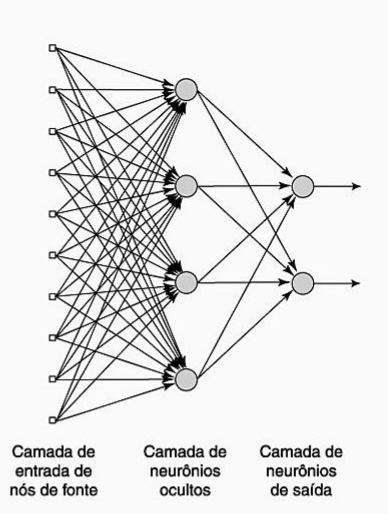
\includegraphics[width=180pt]{dados/figuras/multi_camadas}
  \fonte{\cite{haykin2001}}
  \label{fig:multicamada}
\end{figure}
\item \textbf{Redes recorrentes:} essa classe de arquitetura se diferencia das anteriores pelo fato de possuir pelo menos uma camada com realimentação, ou seja, a saída da camada serve de entrada para a mesma, exemplo \autoref{fig:retroalimentacao}. Os operadores de atraso unitário, representados na imagem pelo símbolo $z^{-1}$, são aplicados nas conexões de realimentação modificando de maneira dinâmica e não linear os valores informados. É dito que a rede possui uma auto-realimentação quando a saída de um neurônio realimenta a sua entrada.
\begin{figure}[H]
  \centering
  \caption{Exemplo de rede retroalimentada.}
  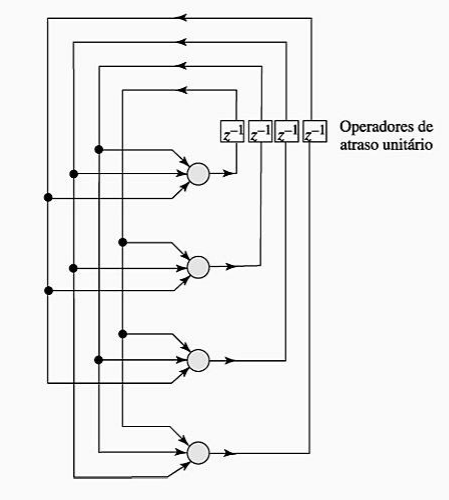
\includegraphics[width=180pt]{dados/figuras/retroalimentacao}
  \fonte{\cite{haykin2001}}
  \label{fig:retroalimentacao}
\end{figure}
\end{itemize}
\section{\textit{Deep learning}}
\textit{Deep learning} pode ser definido como uma hierarquia de "\textit{conceitos}" de aprendizagem, em que "\textit{conceitos}" complexos se originam de grupos formados por "\textit{conceitos}" mais simples. Se representar esses "\textit{conceitos}" em um grafo, é possível ver como um "\textit{conceito}" é montado baseado no outro, como se possuíssem muitas camadas \cite{Goodfellow-et-al-2016}.

\begin{citacao}
    \textit{Deep learning} permite que modelos computacionais compostos de múltiplas camadas de processamento aprendam representações de dados com múltiplos níveis de abstração.
    %[...].
    %        Esses métodos tem drasticamente melhorado o estado-da-arte em reconhecimento de fala, reconhecimento visual de objetos, detecção de objetos e muitos outros domínios como na medicina.
   O  \textit{deep learning} descobre estruturas complexas em vastos conjuntos de dados com o uso do algoritmo de retropropagação para indicar como a máquina deve mudar seus parâmetros internos que são utilizados para computar a representação resultante da camada anterior em cada camada \cite{lecun2015deep}.
\end{citacao}

\par \citeonline{bengio2013representation} categoriza o \textit{deep learning} como um método de aprendizagem de representação (do inglês, \textit{representation learning}). Métodos ditos como \textit{representation learning} são capazes receber dados sem tratamento como entrada e a partir de processamentos internos encontrar automaticamente características relevantes para realizar a classificação. Na qual, para o \textit{deep learning}, cada camada oculta de processamento produz uma nova representação, podendo ser descrito como um método de aprendizado de multi representações. Dessa maneira a entrada pode ser uma imagem, descrita em um mapa de \text{bits}, na qual a primeira camada analisa informações mais superficiais, como contornos ou formas em certas áreas das imagens. Já na segunda camada seriam identificados padrões avaliando certas disposições de bordas ou formas em partes da imagem, ignorando pequenas variações. E na terceira camada seria identificado os padrões que se assemelham a parte de objetos conhecidos, e nas camadas posteriores seriam avaliados uma quantidade maior de padrões até chegar ao ponto de realizar a classificação dos objetos contidos na imagem \cite{lecun2015deep}.

\subsection{Redes neurais convolucionais}
Como descrito por \citeonline{lecun1989backpropagation} redes neurais convolucionais são um tipo especializado de rede neural para processamento de dados que se organizam em grade (ou matriz), tendo como um exemplo de entrada uma imagem, uma matriz de \textit{bits}.
\par Elas possuem o nome de rede convolucional, pois em algumas de suas camadas ocultas ela contém uma camada de convolução. Outro tipo de camada muito utilizada nessas redes é a camada de \textit{pooling} \cite{Goodfellow-et-al-2016}.
\par Uma camada de uma rede neural convolucional geralmente é composta de três fases: a primeira fase onde é aplicada diversas convoluções em paralelo na mesma imagem gerando um conjunto de ativações lineares; a segunda fase propõem a aplicação de uma função de ativação não linear, sendo a unidade linear de correção (do inglês \textit{rectified linear unit}, ReLU) muito utilizada atualmente \cite{lecun2015deep}; e no terceiro e ultimo estágio é utilizado uma função de \textit{pooling} para modificar o dado que será fornecido para a próxima camada.    
\subsubsection{Operação de convolução}
Camadas de convolução são baseadas essencialmente na operação de convolução. Segundo \cite{Goodfellow-et-al-2016}, a operação de convolução é descrita por uma operação que ocorre entre duas funções, podendo ser descrita da seguinte maneira:\[s(t) = (x*w)(t)\] %TODO explicar o valor de t


Em redes convolucionais os argumentos da função de convolução são geralmente compostos pela a entrada de dado ($x$) e o \textit{kernel} ($w$) utilizado para a modificação. Sua saída é um mapa de características (\textit{feature maps}).

\par Assim, a entrada de dados normalmente é uma matriz, nesse caso uma imagem. O \textit{kernel} utilizado também costuma ser uma matriz de parâmetros que podem ser ajustados pelo processo de aprendizagem (retropropagação). E como saída, cria uma matriz da dados com algumas características ressaltadas.

\par A operação de convolução é uma maneira eficiente de descrever transformações para serem aplicadas em áreas menores mantendo a linearidade, em todo o dado de entrada. Como levantado por \citeonline{Goodfellow-et-al-2016}, para realizar uma operação de subtração entre os \textit{pixels} de uma imagem, para serem encontradas as bordas contidas na imagem como visto na \autoref{fig:convolution}, é necessário uma quantidade muito menor de computação para obter o resultado desejado quando é utilizado a convolução.

\begin{figure}[H]
  \centering
  \caption{Exemplo da aplicação de operações para encontrar as bordas verticais de uma imagem. A esquerda a imagem normal em escala cinza e a direita a imagem aplicada a operação subtração dos \textit{pixeis} vizinhos.}
  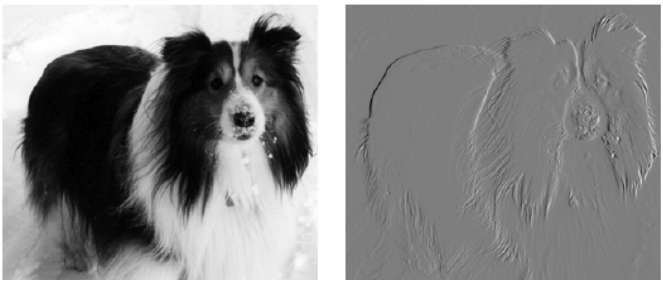
\includegraphics[width=400pt]{dados/figuras/convolution}
  \fonte{\cite{Goodfellow-et-al-2016}}
  \label{fig:convolution}
\end{figure}


\subsubsection{ReLu}

A função de ativação linear (ReLu), vem sendo recomendada a ser utilizada em redes neurais alimentadas adiante \cite{glorot2011deep}. Como visto na \autoref{fig:relu}, a ReLu se mantém muito próxima de uma função linear. Funções ReLus apresentam características que as possibilitam aplicarem as otimizações utilizadas em funções lineares. 
\par Sua função é descrita por pela equação $g(z)=max\{0,z\}$, onde o $z$ no contexto de CNN é a taxa de correção, calculada pelas saídas e as \textit{bias}. 

\begin{figure}[H]
  \centering
  \caption{Gráfico da função de ativação não linear ReLu.}
  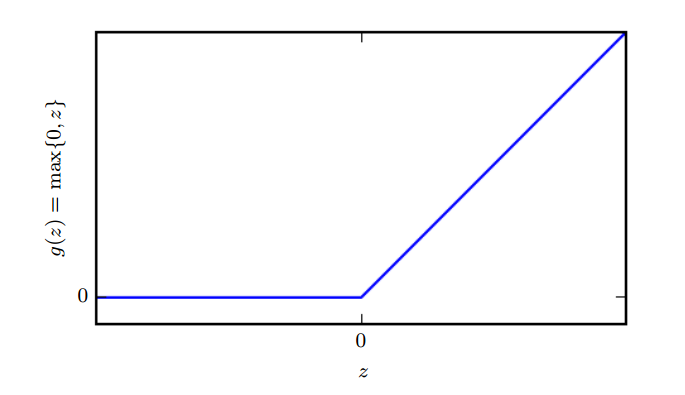
\includegraphics[width=400pt]{dados/figuras/relu}
  \fonte{\cite{Goodfellow-et-al-2016}}
  \label{fig:relu}
\end{figure}

\subsubsection{Operação de \textit{pooling}}
A aplicação da função de \textit{pooling} para modificar o dado de entrada, ajuda a tornar o modelo classificador adaptado a pequenas translações da entrada \cite{Goodfellow-et-al-2016}. Dessa forma a aplicação dessa operação permite identificar se o objeto está contido na imagem independente do local que aparece e da inclinação que apresenta. Essa característica se torna muito eficaz para ser aplicada em redes que necessitam dessa variabilidade de padrões de posição para uma mesma classe.

\par Exemplificando, em uma carta a aplicação da operação de \textit{pooling} permite a rede identificar os números do código postal que estão escrito a mão na carta, mesmo que estes não estejam localizados no mesmo local, ou inclinação de cada respectiva imagem, como exemplo na \autoref{fig:pooling}. 
\begin{figure}[H]
  \centering
  \caption{Exemplo de como é feito a ativação de um neurônio na camada de \textit{pooling}.}
  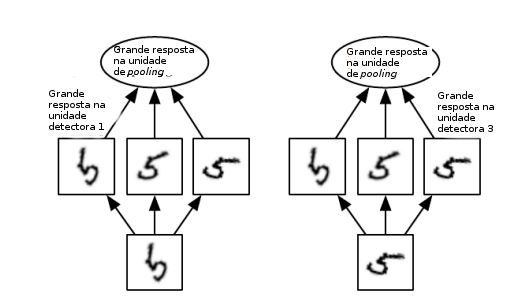
\includegraphics[width=200pt]{dados/figuras/pooling}
  \fonte{\cite{Goodfellow-et-al-2016}}
  \label{fig:pooling}
\end{figure} 

% \subsubsection{Camadas densamente conectadas}

\subsubsection{\textit{Dropout}}
Um dos grandes problemas do uso de CNN é o \textit{overfitting}, que ocorre quando a base disponível para o treino é pequena ou quando a rede neural possui muitas camadas. Uma estratégia utilizada por \citeonline{imaginetArticle} é a aplicação da técnica de \textit{dropout} em algumas camadas da rede.
\par \citeonline{srivastava2014dropout} define o termo \textit{dropout} como a remoção temporária de alguns neurônios da rede, junto com suas conexões de entradas e saídas como é possível visualizar na \autoref{fig:dropout}. Essa operação, que remove virtualmente o neurônio da rede neural, ocorre somente no fase de treino, na qual quando é ativada no neurônio o excluindo nessa execução do processo de aprendizagem da rede.
\begin{figure}[H]
  \centering
  \caption{Exemplo da aplicação do \textit{dropout} em uma rede neural. Na imagem (1) apresenta uma rede normal sem remoção de neurônio. Na imagem (2) mostra a rede com o \textit{dropout} ativado em alguns neurônios, os removendo temporariamente.}
  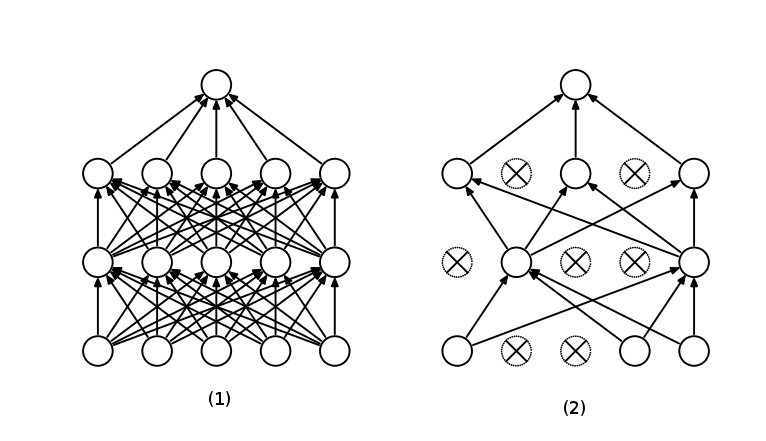
\includegraphics[width=400pt]{dados/figuras/dropout}
  \fonte{\cite{srivastava2014dropout}}
  \label{fig:pooling}
\end{figure} 
\par Essa operação vem com o intuito de reduzir o \textit{overfitting}. A redução do tempo de execução e  o aprendizado de atributos mais relevantes pela rede são outras características que se destacam quando aplicada essa técnica.

% \subsubsection{\textit{Softmax}}

%TODO esplicar sobre dropout e sofmax e fullconected layers         % Revisão de Literatura
% METODOLOGIA------------------------------------------------------------------

\chapter{METODOLOGIA}
\label{chap:metodologia}
%TODO melhorar descrição da sessão
Nessa seção, serão descritas no desenvolvimento dessa monografia, sendo elas a formulação e pré-processamento da base de dados, a configuração da rede neural e sua codificação utilizando o \textit{framework} \textit{keras} \cite{chollet2015keras}, e pesquisas e aplicações de melhorias para a rede neural proposta.

\section{Formulação da base}
No aprendizado de máquina, a base de dados em que serão feitos os treinos e os testes do método escolhido devem possuir um balanceamento na distribuição de amostras por classes, e as amostras de uma mesma classe devem possuir características que as diferenciem das outras amostras de outras classes.

\par Nesse trabalho será feito a classificação de imagens de comida, dessa maneira a base montada contém imagens segregadas em classes como \textit{pizza} e \textit{sushi}. Também foram adicionadas classes de imagens que não estão relacionadas com comida, como \textit{plant}(no português, planta) e \textit{domestic animals}(no português, animais domésticos), visando melhorar o classificador, quando utilizado em bases que possuam imagens não associadas a comida.
\par As imagens utilizadas para a formulação da base de dados desse trabalho foram retiradas das bases de dados \textit{ImageNet}\cite{deng2009imagenet} e \textit{Food-101}\cite{bossard14}. A base \textit{ImageNet} é densamente estruturada e organizada em hierarquia de árvore, facilitando assim encontrar as categorias que estão relacionadas ao tema abordado. Já base \textit{Food-101} é composta de 101 classes de imagens de comida, selecionadas e com um tamanho fixo de 1000 imagens por classe. A precisão de categorização das bases \textit{ImageNet} e \textit{Food-101} são necessárias para a formulação da base de teste deste projeto, tendo em vista que a categorização manual de imagens não seria uma abordagem viável, uma vez que redes neurais convolucionais demandam uma grande quantidade de imagens para um treinamento adequado.  

\par A base formulada possui um total de 16000 imagens separadas em 16 classes, sendo dessas classes 13  relacionadas com comida (\textit{chocolate cake, french fries, hamburger, ice cream, pizza, spaghetti bolognese, sushi,club sandwich, filet mignon, fried rice, hot dog, steak, tacos}) e três não relacionadas com comida (\textit{domestic animal, people, plant}). A diversidade dessas imagens seguem como exemplo na \autoref{fig:imagebase}.
%TODO Alterar essa imagem
\begin{figure}[H]
  \centering
  \caption{Exemplos de imagens encontradas na base de dados.}
  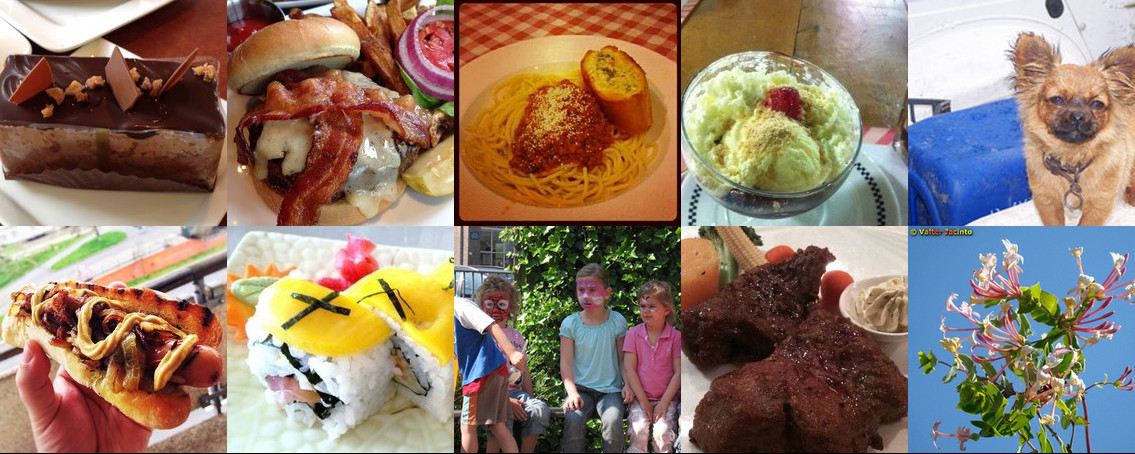
\includegraphics[width=300pt]{dados/figuras/imagembase}
  \fonte{Fonte: imagens retiradas da base \textit{ImageNet}\cite{deng2009imagenet}}
  \label{fig:imagebase}
\end{figure}

\subsection{Pré-processamento}
\par Redes neurais convolucionais requerem de uma grande quantidade de imagens, dessa maneira as entradas fornecidas para a rede neural devem seguir um padrão, onde todas as imagens devem possuir as mesmas dimensões. Assim as imagens foram redimensionadas para 227x227 \textit{pixels}, tendo em vista que é um valor que obteve bons resultados em trabalhos semelhantes \cite{imaginetArticle}. Nas alterações de dimensões das imagens foi realizado um corte nas imagens originais para forçar uma formato quadrado antes de ser aplicado o redimensionamento, preservando os formatos das imagens.
\par Para a realização dos treinos e testes com a rede neural a base de dados foi separada em dados de treino e dados de teste. Onde 70\% das imagens (11200 imagens) de cada classe serão utilizadas para o treino da rede neural, e os 30\% das imagens restantes  (4800 imagens) serão utilizadas para a fase de teste da rede neural.

%TODO Adicionar tabela com as classes a quantidade de treino, teste e total

\section{Configuração da Rede Neural}
A configuração da rede neural convolucional utilizada nesse projeto é fundamentada na rede neural \textit{AlexNet} definida por \citeonline{imaginetArticle}. Essa rede utiliza de 8 camadas ocultas de processamento, sendo cinco camadas convolucionais e três camadas fortemente conectadas. Tendo em vista que a rede utilizada como exemplo foi estruturada para classificar mil classes, é necessário fazer algumas adaptações na rede para classificar uma quantidade menor de classes, uma dessas alterações seria a modificação da função \textit{softmax} para obter o resultado da classificação na última camada.
\par A primeira camada de convolução da rede irá separar a entrada, uma imagem de 227x227X3 em 96 núcleos de 11x11x3 (com uma distancia de 4 \textit{pixels} entre os centros das imagens vizinhas), onde cada imagem gerada será processada separadamente. Após essa camada é aplicada uma camada de \textit{max pooling}.
\par A segunda camada convolucional tem como entrada a saída da primeira camada convolucional normalizada e com \textit{pooling} aplicado, essa entrada é filtrada em 256 núcleos de 5x5x48. Após esse camada também é aplicado uma camada de \textit{max pooling}.
\par A terceira camada convolucional possui 384 núcleos de 3x3x256 que são conectados a entrada fornecida pela saída da segunda camada convolucional normalizada e aplicado o \textit{pooling}. As conexões entre a terceira, quarta e quinta camada convolucional, não possuem nenhuma operação de \textit{pooling} entre si. 
\par Assim a quarta camada convolucional possui 384 núcleos de 3x3x192 e a quinta camada possui 256 núcleos de 3x3x192. Após a quinta camada convolucional é aplicado uma camada de \textit{max pooling}.
\par A duas camadas seguintes são camadas fortemente conectadas com 4096 neurônios cada. E por fim uma camada com 10 neurônios (um neurônio para cada classe) fortemente conectada com a operação de \textit{softmax} para obter a predição da entrada.

%TODO adicionar uma imagem para descrever a arquitetura da rede neural

\par Está sendo utilizado o \textit{framework} \textit{Keras} \cite{chollet2015keras} para descrever a rede neural. \textit{Keras} é um \textit{framework} em \textit{python} para execução de redes neurais utilizando \textit{GPU}(\textit{Graphics Processing Unit}). Com o \textit{keras} é possível configurar em alto nível uma rede neural, abstraindo a complexidade da descrição e implementação das rotinas de execução das camadas. Como exemplo de implementação temos a Figura \ref{fig:conv_keras}, contendo a codificação da primeira e segunda camada da rede neural proposta.

\begin{figure}[H]
  \centering
  \caption{Trecho de código com implementação utilizando o \textit{framework} \textit{keras} das duas primeiras camadas convolucionais da rede neural, contendo a definição da entrada e as implementações das camadas de transição entre as camadas de convolução um e dois.}
  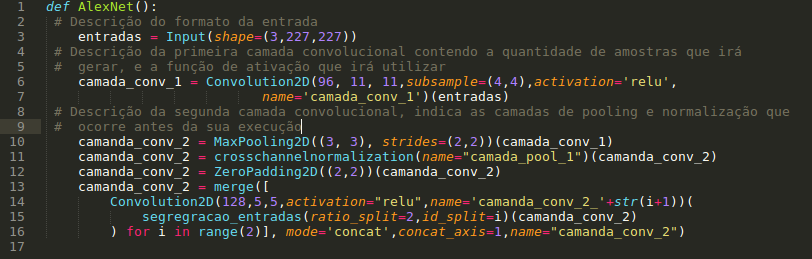
\includegraphics[width=400pt]{dados/figuras/exemplo_keras}
  \caption*{Fonte: Imagem produzida pelo autor (2017).}
  \label{fig:conv_keras}
\end{figure}


\section{Melhorias para a rede neural proposta}

Melhorias no desempenho de redes neurais podem ser aplicadas em diversas etapas do processo de aprendizado e classificação. O aumento da base de treino, definir camadas serão para serem treinadas em determinadas épocas, a inicialização dos pesos da rede neural com valores de uma rede treinada com uma quantidade maior de amostras e o aprimoramento dos parâmetros de configuração da rede, são métodos que podem ser utilizados para aprimorar sua performance de classificação.

%colocar referencia das sessões que foram descritos as tecnicas utilizadas 
\par Nesse projeto foram aplicadas técnicas para a melhora na classificação, sendo elas
%técnicas o ajuste empírico da taxa de descarte de neurônios nas camadas totalmente conectadas,
o aumento dos dados na base de treino e a inicialização dos pesos da rede neural com pesos de uma rede já treinada. Essas técnicas são descritas mais detalhadamente nas seções a seguir.

\subsection{\textit{Data augmentation}}
Uma técnica que vem sendo muito utilizada no para a redução do \textit{overfitting} na fase de treino de uma rede neural é a \textit{data augmentation} \cite{cui2015data}. 
Os dados da base são ligeiramente modificados, para obter aumento na quantidade de amostras.
%TODO colocar referencia aki
Essas mudanças nas imagens podem ser inversões nos eixos, pequenas rotações, aproximações em certas partes das imagens ou até a aplicação da imagem em escala cinza.
Essa técnica tem o propósito de aumentar a quantidade de amostras em que serão realizados os treinos, buscando evitar um \textit{overfitting}.
\par Nesse projeto foi utilizada a técnica de \textit{data augmentation} aplicando inversão da imagem no eixo $y$, realizando um zoom de aproximação ou distanciamento de até 20\% da imagem e aplicado uma taxa de inclinação de até 0,2 radianos. As imagens são geradas com a combinação das transformações possíveis informadas, criando nove imagens para cada imagem de treino como representado na \autoref{fig:data_augmentation}. Essas imagens são geradas durante a execução do treino da rede e são armazenadas em memória.

%TODO incluir aki a imagem de data augmentation

\subsection{Inicialização dos pesos}
Uma rede neural treinado do inicio ao fim, tem seus pesos inicializados de maneira aleatória e conforme vai realizando suas predições os pesos são corrigidos para melhorar o poder de classificação. A inicialização dos pesos da rede neural com valores obtidos a partir de uma rede treinada, vem sendo utilizado como maneira de melhorar a classificação. 
%TODO colocar aki referencia de inicialização dos pesos
Geralmente os pesos vem de redes que treinaram uma quantidade muito grande de dados, conseguindo de certa forma transferir o aprendizado obtido para a rede que está inicializando os pesos.
Nesse projeto foi realizado a inicialização dos pesos da rede neural, utilizando os pesos obtidos no treinamento da rede desenvolvida por \citeonline{imaginetArticle}.

% \subsection{Congelamento de camadas}



% \par O aprimoramento da rede neural convolucional pode ser feito por meio da utilização de parâmetros já treinados da rede neural, \cite{Girshick_2014_CVPR} descreve esse método como um pré-treino da rede, a preparando para a sua real tarefa. Podendo assim utilizar os pesos treinados em \cite{imaginetArticle} para um aperfeiçoamento da rede.
% \par Outro método utilizado para a melhora do resultado e redução do \textit{overfit}(quando um classificador não produz resultados bons de classificação para entradas diferentes das contidas na base de dados) é o de poda na rede \cite{NIPS2015_5784}. Onde os pesos de conexão podem ser agrupados por meio de \textit{hash} identificando parâmetros similares entre eles, tendo assim um parâmetro para cada grupo de peso.
% \par Uma técnica utilizada para o aumento da base de dados é o \textit{data aumentation}, onde os dados da base são ligeiramente modificados, para obter um crescimento da base. Essa técnica é aplica para reduzir o \textit{overfit} e aumentar a base de teste. Essas mudanças nas imagens podem ser inversões das imagens, pequenas rotações ou aproximações em certas partes das imagens.


%Melhorias no desempenho de redes neurais podem ser aplicadas em diversas etapas do processo de aprendizado e classificação. O aumento da base de treino por meio de técnicas de \textit{data augmentation} \cite{imaginetArticle}\cite{cui2015data}, definir quais camadas serão treinadas em determinadas épocas utilizando a técnica conhecida como \textit{layer-wise} \cite{tajbakhsh2016convolutional}, a inicialização dos pesos da rede com valores de uma rede treinada com uma quantidade maior de amostras técnica conhecida como \textit{transfer learning} (em português, transferência de aprendizagem)\cite{Girshick_2014_CVPR}, são métodos                     % Metodologia
% RESULTADOS-------------------------------------------------------------------

\chapter{ANÁLISE E DISCUSSÃO DOS RESULTADOS}

% Cada capítulo deve conter uma pequena introdução (tipicamente, um ou dois parágrafos) que deve deixar claro /o objetivo e o que será discutido no ecapítulo, bem como a organização do capítulo.

Nesta seção estão descritos os resultados obtidos a partir dos testes realizados na a rede neural convolucional proposta, apresentando os resultados obtidos com a variação da aplicação das técnicas propostas.
 %A métrica utilizada para avaliar os modelos foi a acurácia, que determina a porcentagem de acerto do classificador.%TODO definir melhor a metrica
 Os testes foram iniciados a partir da rede neural convolucional sem nenhuma alteração, seguindo para a inclusão das alterações na base e melhorias na rede, com o fim de avaliar os resultados obtidos e determinar o modelo com a melhor acurácia.

\par Nos teste iniciais realizados foram identificados que a partir de 80 épocas de execução não ocorria nenhuma modificação nas fases de treino e teste, sempre mantendo,mantendo uma faixa de variação constante. Dessa maneira foi definido como padrão a quantidade de 80 épocas para a execução dos testes. A escolha dos parâmetros da rede como a taxa de \textit{dropout}, foram definidos com base na rede descrita por \cite{imaginetArticle}. Como abordagem de melhoria a taxa de \textit{dropout} foi otimizada para o modelo proposto por base de testes empíricos.
%\section{Acurácia}


\section{Modelo inicial}
O teste realizado com o modelo inicial proposto utilizando da base de dados sem modificação obteve um resultado de 94,02\% de acurácia na base de treino e 53,6\% na base de teste, como apresentado na \autoref{tab:resultado1}. Com esses valores é possível dizer que ocorreu um \textit{overfitting} no modelo sobre as amostras da base de treino. Com o gráfico apresentado na \autoref{fig:resultado1} é visto que a acurácia da fase de teste a partir de 42 épocas mantém valores constantes, não apresentando uma ganho expressivo, diferente da acurácia obtida na fase de treino que mantém uma curva crescente.

\begin{table}[H]
    \centering
    \caption{Resultado da execução do modelo inicial sem as aplicações das melhorias \textit{data augmentation} e inicialização dos pesos.
    \label{tab:resultado1}}
    \begin{tabular}{ccc}
        \toprule
              & Fase de treino & Fase de Teste \\
        \midrule
            Modelo inicial & 94,02\% & 53,6\%  \\
        \bottomrule
    \end{tabular}
\end{table}


\begin{figure}[H]
  \centering
  \caption{Gráfico contendo a acurácia obtida na fase de treino e teste de cada época do modelo de rede neural inicialmente proposta sem a aplicação de técnicas de melhorias.}
  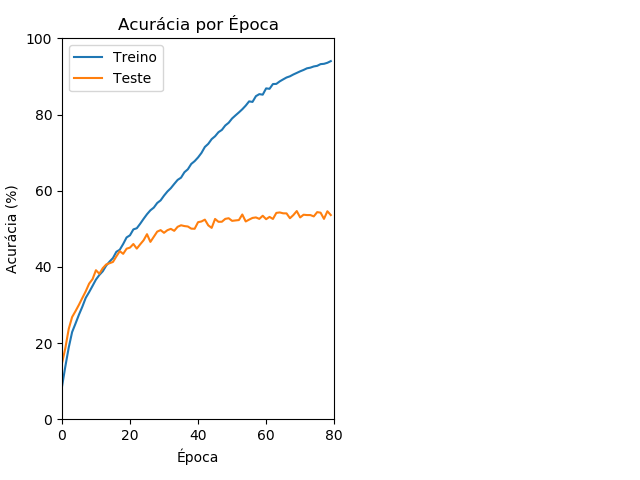
\includegraphics[width=300pt]{dados/figuras/resultado1}
  \label{fig:resultado1}
\end{figure}

\section{Modelos com \textit{data augmentation} e inicialização dos pesos}
Também foram realizados testes com as estratégias de melhorias da rede neural, com o objetivo de reduzir o \textit{overfitting} na rede neural. Foram realizados três testes: o teste aplicando a técnica de \textit{data augmentation}; o teste aplicando a técnica de inicialização dos pesos a partir dos valores treinados na rede desenvolvida por \citeonline{imaginetArticle}; e o teste aplicando ambas as técnicas. 

\par Como informado na \autoref{tab:resultado2} as acurácias obtidas na fase de teste e treino, respectivamente, apenas com \textit{data augmentation} foram de 58,23\% e 71,66\%, vendo com essa mudança uma redução significativa do \textit{overfitting} na rede, além de uma melhora da acurácia na fase de teste.

\begin{table}[H]
    \centering
    \caption{Resultados da execução do modelo inicialmente proposto sem a aplicação de tecnicas de melhorias.
    \label{tab:resultado2}}
    \begin{tabular}{ccc}
        \toprule
              & Fase de treino & Fase de Teste \\
        \midrule
            Modelo com \textit{data augmentation} & 71,66\% & 58,23\%  \\
            Modelo com inicialização dos pesos & 99,63\% & 68,08\%  \\
            Modelo com \textit{data augmentation} e inicialização dos pesos & 98,18\% & 71,77\%  \\
        \bottomrule
    \end{tabular}
\end{table}


\begin{figure}[H]
  \centering
  \caption{Gráficos contendo as acurácias obtidas nas fases de treino e teste dos modelos com as melhorias aplicadas. No gráfico (1) apresenta os resultados do teste com a utilização de \textit{data augmentation}. No gráfico (2) apresentado os resultados do teste com a inicialização dos pesos a partir de uma rede treinada. E no gráfico (3) apresenta os resultados obtidos com o modelo com a técnica de \textit{data augmentation} e inicialização dos pesos.}
  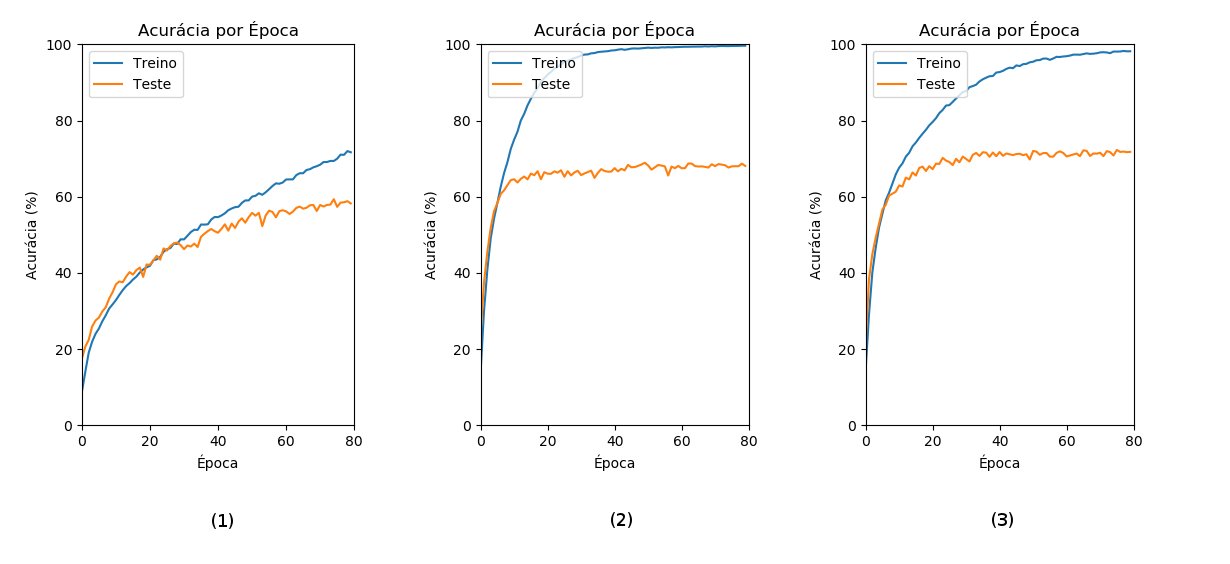
\includegraphics[width=500pt]{dados/figuras/resultado2}
  \label{fig:resultado2}
\end{figure}

\par O teste realizado com a inicialização dos pesos obteve um resultado mais expressivo se comparado com o teste apenas com \textit{data augmentation} obtendo as acurácias na fase de teste e treino, respectivamente, de 68,08\% e 99,63\%. Com a aplicação dessa técnica foi obtido uma melhora significativa na acurácia se comparado com o modelo inicial e o modelo com \textit{data augmentation}, mas assim como no modelo inicial esse modelo apresenta \textit{overfitting} na fase de treino, como é possível observar nos gráficos (2) da \autoref{fig:resultado2}, a partir da época 20 a acurácia da fase de teste permanece estável e a fase de treino continua crescendo até atingir valores próximos a 100\%.

\par Com o intuito de solucionar o problema de \textit{overfitting} e obter melhoria na classificação, foi realizado o teste utilizando as duas técnicas. A acurácia obtida na fase de treino foi de 98,18\% e na fase de teste obteve um valor de 71,77\%, apresentando o melhor resultado entre os três testes realizados como pode ser observado no gráfico comparativo na \autoref{fig:resultado2all}.% TODO colocar referencias que apresentam melhoria em modelos aplicados  data augmentantion e inicialização de pesos
\begin{figure}[H]
  \centering
  \caption{Gráficos contendo as acurácias obtidas nas fases de teste dos modelos com as melhorias aplicadas.}
  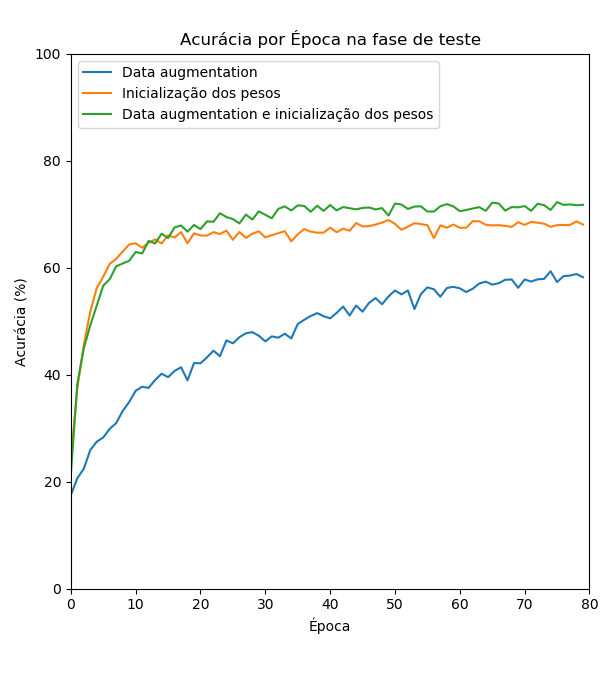
\includegraphics[width=500pt]{dados/figuras/resultado2_all}
  \label{fig:resultado2all}
\end{figure}
 
\section{Aprimoramento da taxa de \textit{dropout}}
Foram realizados testes com a taxa de \textit{dropout} buscando diminuir o \textit{overfitting} na rede. A taxa de \textit{dropout} foi variada de 50\% a 90\%, com intervalos de 10\% entre cada teste. O modelo utilizado para a execução dos foi o proposto com a aplicação de \textit{data augmentation} e inicialização dos pesos. Como pode ser verificado na \autoref{tab:resultado3} a taxa de 80\% foi a que apresentou melhor resultado com uma acurácia de 74,56\% na fase de teste e 93,96\% de acurácia na fase de treino.

\begin{table}[H]
    \centering
    \caption{Resultados da execução com a variação na taxa de \textit{dropout}.
    \label{tab:resultado3}}
    \begin{tabular}{ccc}
        \toprule
             Taxa de \textit{dropout} (\%) & Fase de treino & Fase de Teste \\
        \midrule
            Modelo com taxa de 60\% & 97,78\% & 72\%  \\
            Modelo com taxa de 70\% & 96,61\% & 72,77\%  \\
            Modelo com taxa de 80\% & 93,96\% & 74,56\%  \\
            Modelo com taxa de 90\% & 95,37\% & 72,24\%  \\
        \bottomrule
    \end{tabular}
\end{table}


\par A partir da \autoref{tab:resultado3} é possível concluir que os teste realizado com a taxa de \textit{dropout} 80\% apresentou a maior acurácia na fase de teste e  apresentando a menor diferença entre os resultado da fase de treino e teste, conseguindo melhorar o \textit{overfitting} que ocorre na rede. 

                    % Resultados
% % ORIENTAÇÕES GERAIS------------------------------------------------------------


% SOBRE AS ILUSTRAÇÕES----------------------------------------------------------
\chapter{SOBRE AS ILUSTRAÇÕES}
\label{chap:apSobreIlust}

A seguir exemplifica-se como inserir ilustrações no corpo do trabalho. As ilustrações serão indexadas automaticamente em suas respectivas listas. A numeração sequencial de figuras, tabelas e equações também ocorre de modo automático.

Referências cruzadas são obtidas através dos comandos \verb|\label{}| e \verb|\ref{}|. Sendo assim, não é necessário por exemplo, saber que o número de certo capítulo é \ref{chap:fundamentacaoTeorica} para colocar o seu número no texto. Outra forma que pode ser utilizada é esta: \autoref{chap:fundamentacaoTeorica}, facilitando a inserção, remoção e manejo de elementos numerados no texto sem a necessidade de renumerar todos esses elementos.

% FIGURAS-----------------------------------------------------------------------
\chapter{FIGURAS}
\label{chap:figuras}

Exemplo de como inserir uma figura. A \autoref{fig:figura-exemplo1} aparece automaticamente na lista de figuras. Para saber mais sobre o uso de imagens no \LaTeX{} consulte literatura especializada \cite{Goossens2007}.

Os arquivos das figuras devem ser armazenados no diretório de "/dados".

\begin{figure}[!htb]
    \centering
    \caption{Exemplo de Figura}
    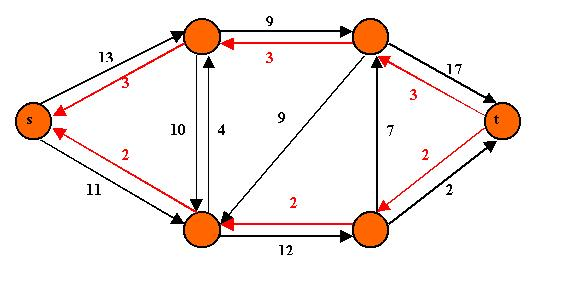
\includegraphics[width=0.5\textwidth]{./dados/figuras/figura1}
    \fonte{\citeonline{IRL2014}}
    \label{fig:figura-exemplo1}
\end{figure}

% QUADROS E TABELAS---------------------------------------------------------------
\chapter{QUADROS E TABELAS}
\label{chap:tabelas}

Exemplo de como inserir o \autoref{qua:quadro-exemplo1} e a \autoref{tab:tabela-exemplo1}. Ambos aparecem automaticamente nas suas respectivas listas. Para saber mais informações sobre a construção de tabelas no \LaTeX{} consulte literatura especializada \cite{Mittelbach2004}.

Ambos os elementos (Quadros e Tabelas) devem ser criados em arquivos separados para facilitar manutenção e armazenados no diretório de "/dados".

\begin{quadro}[!htb]
    \centering
    \caption{Exemplo de Quadro.\label{qua:quadro-exemplo1}}
    \begin{tabular}{|p{7cm}|p{7cm}|}
        \hline
        \textbf{BD Relacionais} & \textbf{BD Orientados a Objetos} \\
        \hline
        Os dados são passivos, ou seja, certas operações limitadas podem ser automaticamente acionadas quando os dados são usados. Os dados são ativos, ou seja, as solicitações fazem com que os objetos executem seus métodos. & Os processos que usam dados mudam constantemente. \\
        \hline
    \end{tabular}
    \fonte{\citeonline{Barbosa2004}}
\end{quadro}


A diferença entre quadro e tabela está no fato que um quadro é formado por linhas horizontais e verticais. Deve ser utilizado quando o conteúdo é majoritariamente não-numérico. O número do quadro e o título vem acima do quadro, e a fonte, deve vir abaixo. E Uma tabela é formada apenas por linhas verticais. Deve ser utilizada quando o conteúdo é majoritariamente numérico. O número da tabela e o título vem acima da tabela, e a fonte, deve vir abaixo, tal como no quadro.

\begin{table}[!htb]
    \centering
    \caption[Resultado dos testes]{Resultado dos testes.
    \label{tab:tabela-exemplo1}}
    \begin{tabular}{rrrrr}
        \toprule
            & Valores 1 & Valores 2 & Valores 3 & Valores 4 \\
        \midrule
            Caso 1 & 0,86 & 0,77 & 0,81 & 163 \\
            Caso 2 & 0,19 & 0,74 & 0,25 & 180 \\
            Caso 3 & 1,00 & 1,00 & 1,00 & 170 \\
        \bottomrule
    \end{tabular}
    \fonte{\citeonline{Barbosa2004}}
\end{table}


% EQUAÇÕES-----------------------------------------------------------------------
\chapter{EQUAÇÕES}
\label{chap:equacoes}

Exemplo de como inserir a \autoref{eq:equacao-exemplo1} e a Eq. \ref{eq:equacao-exemplo2} no corpo do texto \footnote{Deve-se atentar ao fato de a formatação das equações ficar muito boa esteticamente.}. Observe que foram utilizadas duas formas distintas para referenciar as equações.

\begin{equation}
    X(s) = \int\limits_{t = -\infty}^{\infty} x(t) \, \text{e}^{-st} \, dt
    \label{eq:equacao-exemplo1}
\end{equation}

\begin{equation}
    F(u, v) = \sum_{m = 0}^{M - 1} \sum_{n = 0}^{N - 1} f(m, n) \exp \left[ -j 2 \pi \left( \frac{u m}{M} + \frac{v n}{N} \right) \right]
    \label{eq:equacao-exemplo2}
\end{equation}

% ALGORITMOS-----------------------------------------------------------------------
\chapter{ALGORITMOS}
\label{chap:algoritmos}

Exemplo de como inserir um algoritmo. Para inserção de algoritmos utiliza-se o pacote {\ttfamily algorithm2e} que já está devidamente configurado dentro do template.

Os algoritmos devem ser criados em arquivos separados para facilitar manutenção e armazenados no diretório de "/dados".\\
\\

\begin{algorithm}
    \caption{Exemplo de Algoritmo}
    \KwIn{o número $n$ de vértices a remover, grafo original $G(V, E)$}
    \KwOut{grafo reduzido $G'(V,E)$}
    $removidos \leftarrow 0$ \\
    \While {removidos $<$ n } {
        $v \leftarrow$ Random$(1, ..., k) \in V$ \\
            \For {$u \in adjacentes(v)$} {
                remove aresta (u, v)\\
                $removidos \leftarrow removidos + 1$\\
            }
            \If {há  componentes desconectados} {
                remove os componentes desconectados\\
            }
        }
\end{algorithm}


% SOBRE AS LISTAS--------------------------------------------------------------------
\chapter{SOBRE AS LISTAS}
\label{chap:apSobreLista}

Para construir listas de "\textit{bullets}"{} ou listas enumeradas, inclusive listas aninhadas, é utilizado o pacote \verb|paralist|.

Exemplo de duas listas não numeradas aninhadas, utilizando o comando \verb|\itemize|. Observe a indentação, bem como a mudança automática do tipo de "\textit{bullet}"{} nas listas aninhadas.

\begin{itemize}
    \item item não numerado 1
    \item item não numerado 2
    \begin{itemize}
        \item subitem não numerado 1
        \item subitem não numerado 2
        \item subitem não numerado 3
    \end{itemize}
    \item item não numerado 3
\end{itemize}

Exemplo de duas listas numeradas aninhadas, utilizando o comando \verb|\enumerate|. Observe a numeração progressiva e indentação das listas aninhadas.

\begin{enumerate}
    \item item numerado 1
    \item item numerado 2
    \begin{enumerate}
        \item subitem numerado 1
        \item subitem numerado 2
        \item subitem numerado 3
    \end{enumerate}
    \item item numerado 3
\end{enumerate}

% SOBRE AS CITAÇÕES E CHAMADAS DE REFERÊNCAS----------------------------------------------
\chapter{SOBRE AS CITAÇÕES E CHAMADAS DE REFERÊNCAS}
\label{chap:apSobreCita}

Citações são trechos de texto ou informações obtidas de materiais consultadss quando da elaboração do trabalho. São utilizadas no texto com o propósito de esclarecer, completar e embasar as ideias do autor. Todas as publicações consultadas e utilizadas (por meio de citações) devem ser listadas, obrigatoriamente, nas referências bibliográficas, para preservar os direitos autorais. São classificadas em citações indiretas e diretas.

% CITAÇÕES INDIRETAS-----------------------------------------------------------------------
\chapter{CITAÇÕES INDIRETAS}
\label{chap:citacoesLivres}

É a transcrição, com suas próprias palavras, das idéias de um autor, mantendo-se o sentido original. A citação indireta é a maneira que o pesquisador tem de ler, compreender e gerar conhecimento a partir do conhecimento de outros autores. Quanto à chamada da referência, ela pode ser feita de duas maneiras distintas, conforme o nome do(s) autor(es) façam parte do seu texto ou não. Exemplo de chamada fazendo parte do texto:\\
\\Enquanto \citeonline{Maturana2003} defendem uma epistemologia baseada na biologia. Para os autores, é necessário rever \ldots.\\

A chamada de referência foi feita com o comando \verb|\citeonline{chave}|, que produzirá a formatação correta.

A segunda forma de fazer uma chamada de referência deve ser utilizada quando se quer evitar uma interrupção na sequência do texto, o que poderia, eventualmente, prejudicar a leitura. Assim, a citação é feita e imediatamente após a obra referenciada deve ser colocada entre parênteses. Porém, neste caso específico, o nome do autor deve vir em caixa alta, seguido do ano da publicação. Exemplo de chamada não fazendo parte do texto:\\
\\Há defensores da epistemologia baseada na biologia que argumentam em favor da necessidade de \ldots \cite{Maturana2003}.\\

Nesse caso a chamada de referência deve ser feita com o comando \verb|\cite{chave}|, que produzirá a formatação correta.

% CITAÇÕES DIRETAS-----------------------------------------------------------------------
\chapter{CITAÇÕES DIRETAS}
\label{chap:citacoesLiterais}

É a transcrição ou cópia de um parágrafo, de uma frase, de parte dela ou de uma expressão, usando exatamente as mesmas palavras adotadas pelo autor do trabalho consultado.

Quanto à chamada da referência, ela pode ser feita de qualquer das duas maneiras já mencionadas nas citações indiretas, conforme o nome do(s) autor(es) façam parte do texto ou não. Há duas maneiras distintas de se fazer uma citação direta, conforme o trecho citado seja longo ou curto.

Quando o trecho citado é longo (4 ou mais linhas) deve-se usar um parágrafo específico para a citação, na forma de um texto recuado (4 cm da margem esquerda), com tamanho de letra menor e espaçamento entrelinhas simples. Exemplo de citação longa:
\\\begin{citacao}
    Desse modo, opera-se uma ruptura decisiva entre a reflexividade filosófica, isto é a possibilidade do sujeito de pensar e de refletir, e a objetividade científica. Encontramo-nos num ponto em que o conhecimento científico está sem consciência. Sem consciência moral, sem consciência reflexiva e também subjetiva. Cada vez mais o desenvolvimento extraordinário do conhecimento científico vai tornar menos praticável a própria possibilidade de reflexão do sujeito sobre a sua pesquisa \cite[p.~28]{Silva2000}.
\end{citacao}

Para fazer a citação longa deve-se utilizar os seguintes comandos:
\begin{verbatim}
\begin{citacao}
<texto da citacao>
\end{citacao}
\end{verbatim}

No exemplo acima, para a chamada da referência o comando \verb|\cite[p.~28]{Silva2000}| foi utilizado, visto que os nomes dos autores não são parte do trecho citado. É necessário também indicar o número da página da obra citada que contém o trecho citado.

Quando o trecho citado é curto (3 ou menos linhas) ele deve inserido diretamente no texto entre aspas. Exemplos de citação curta:\\
\\A epistemologia baseada na biologia parte do princípio de que "assumo que não posso fazer referência a entidades independentes de mim para construir meu explicar" \cite[p.~35]{Maturana2003}.\\
\\A epistemologia baseada na biologia de \citeonline[p.~35]{Maturana2003} parte do princípio de que "assumo que não posso fazer referência a entidades independentes de mim para construir meu explicar".

% DETALHES SOBRE AS CHAMADAS DE REFERÊNCIAS---------------------------------------------------------
\chapter{DETALHES SOBRE AS CHAMADAS DE REFERÊNCIAS}
\label{chap:referUtilizadas}

Outros exemplos de comandos para as chamadas de referências e o resultado produzido por estes:\\
\\\citeonline{Maturana2003} \ \ \  \verb|\citeonline{Maturana2003}|\\
\citeonline{Barbosa2004} \ \ \   \verb|\citeonline{Barbosa2004}|\\
\cite[p.~28]{Silva2000} \ \ \  \verb|\cite[p.~28]{Silva2000}|\\
\citeonline[p.~33]{Silva2000} \ \ \   \verb|\citeonline[p.~33]{v}|\\
\cite[p.~35]{Maturana2003} \ \ \   \verb|\cite[p.~35]{Maturana2003}|\\
\citeonline[p.~35]{Maturana2003} \ \ \   \verb|\citeonline[p.~35]{Maturana2003}|\\
\cite{Barbosa2004,Maturana2003} \ \ \   \verb|\cite{Barbosa2004,Maturana2003}|\\

% SOBRE AS REFERÊNCIAS BIBLIOGRÁFICAS-------------------------------------------------------
\chapter{SOBRE AS REFERÊNCIAS BIBLIOGRÁFICAS}
\label{chap:apSobreRefer}

A bibliografia é feita no padrão \textsc{Bib}\TeX{}. As referências são colocadas em um arquivo separado. Neste template as referências são armazenadas no arquivo "base-referencias.bib".

Existem diversas categorias documentos e materiais componentes da bibliografia. A classe abn\TeX{} define as seguintes categorias (entradas):

\begin{verbatim}
@book
@inbook
@article
@phdthesis
@mastersthesis
@monography
@techreport
@manual
@proceedings
@inproceedings
@journalpart
@booklet
@patent
@unpublished
@misc
\end{verbatim}

Cada categoria (entrada) é formatada pelo pacote \citeonline{abnTeX22014d} de uma forma específica. Algumas entradas foram introduzidas especificamente para atender à norma \citeonline{NBR6023:2002}, são elas: \verb|@monography|, \verb|@journalpart|,\verb|@patent|. As demais entradas são padrão \textsc{Bib}\TeX{}. Para maiores detalhes, refira-se a \citeonline{abnTeX22014d}, \citeonline{abnTeX22014b}, \citeonline{abnTeX22014c}.

% NOTAS DE RODAPÉ--------------------------------------------------------------------------
\chapter{NOTAS DE RODAPÉ}
\label{chap:notasRodape}

As notas de rodapé pode ser classificadas em duas categorias: notas explicativas\footnote{é o tipo mais comum de notas que destacam, explicam e/ou complementam o que foi dito no corpo do texto, como esta nota de rodapé, por exemplo.} e notas de referências. A notas de referências, como o próprio nome ja indica, são utilizadas para colocar referências e/ou chamadas de referências sob certas condições.

                   % Capítulo com Orientações de uso do Template
% CONCLUSÃO--------------------------------------------------------------------

\chapter{CONCLUSÃO}
\label{chap:conclusao}

A tarefa de classificação de imagem vem sendo um dos grandes desafios na área de visão computacional. A utilização do \textit{deep learning}, com CNN, para a classificação de imagens vem sendo utilizado desde 2012 e vem atualizando o estado da arte nessa área. Neste trabalho utilizamos de CNN para realizar a classificação de imagens de comida, utilizando técnicas de \textit{data augmentation} e inicialização dos pesos da rede para obter uma melhor classificação e solucionar o \textit{overfitting}, uns dos grandes problemas no uso de CNN.
\par O \textit{overfitting} se mostra o grande obstaculo no uso de CNNs. Uma base de treino muito pequena ou uma rede neural muito profunda~são possíveis causas do \textit{overfitting}. A aplicação de técnicas para aumento da base de dados e a utilização do \textit{dropout} em algumas camadas da rede são medidas que reduzem o \textit{overfitting}, conforme foi aplicado e constatado neste trabalho.
\par \textit{Data augmentation} vem sendo aplicado nos modelos de classificação que utilizam CNN. A aplicação do \textit{data augmentation} na base foi com o objetivo de modificar ligeiramente as imagens originais. Também foi utilizado para melhorar o resultado de classificação a inicialização dos pesos da rede com os valores obtidos a partir de um rede já treinada, ao invés de realizar a inicialização com valores aleatórios.   
\par Nos experimentos realizados o emprego da técnica de \textit{data augmentation}, como relatado por outros trabalhos, obteve um resultado expressivo para realizar a redução do \textit{overfitting}, além que alcançar uma melhora na acurácia. A aplicação em conjunto do \textit{data augmentation}, inicialização dos pesos e otimização da taxa de \textit{dropout} obteve uma resultado de 74,56\% de acurácia, aumentando em 20,96\% a acurácia se comparado com o modelo proposto sem as melhorias (53,6\% de acurácia).
\par Outra abordagem que pode ser realizada futuramente é utilizar o modelo para realizar a extração das características em conjunto com um outro classificado como SVM (do inglês \textit{suport vector machine}) para realizar a predição. A aplicação de vetores de dissimilaridade nas características extraídas com a CNN para a classificação seria outro caminho a ser abordado. Otimizações de outros parâmetros da rede como a taxa de aprendizagem e o estudo de outras arquiteturas de CNN como a \textit{GoogLeNet} \cite{szegedy2015going} para melhorar o desempenho do classificador.                 			   % Conclusão

\postextual
% % INSERE ELEMENTOS PÓS-TEXTUAIS
% REFERÊNCIAS------------------------------------------------------------------

% Carrega o arquivo "base-referencias.bib" e extrai automaticamente as referências citadas

\bibliography{./base-referencias}
\bibliographystyle{abntex2-alf} % Define o estilo ABNT para formatar a lista de referências
% OBSERVAÇÕES------------------------------------------------------------------
% Este arquivo não precisa ser alterado.
           			   % Referências
% % APÊNDICES--------------------------------------------------------------------

\begin{apendicesenv}
\partapendices

% Primeiro apêndice------------------------------------------------------------
\chapter{Nome do apêndice} % Edite para alterar o título deste apêndice
\label{chap:apendiceA}

Lembre-se que a diferença entre apêndice e anexo diz respeito à autoria do texto e/ou material ali colocado.

Caso o material ou texto suplementar ou complementar seja de sua autoria, então ele deverá ser colocado como um apêndice. Porém, caso a autoria seja de terceiros, então o material ou texto deverá ser colocado como anexo.

Caso seja conveniente, podem ser criados outros apêndices para o seu trabalho acadêmico. Basta recortar e colar este trecho neste mesmo documento. Lembre-se de alterar o "label"{} do apêndice.

Não é aconselhável colocar tudo que é complementar em um único apêndice. Organize os apêndices de modo que, em cada um deles, haja um único tipo de conteúdo. Isso facilita a leitura e compreensão para o leitor do trabalho.

% Novo apêndice----------------------------------------------------------------
\chapter{Nome do outro apêndice}
\label{chap:apendiceB}

conteúdo do novo apêndice

\end{apendicesenv}
             			   % Apêndices
% % ANEXO------------------------------------------------------------------------

\begin{anexosenv}
\partanexos

% Primeiro anexo---------------------------------------------------------------
\chapter{Nome do anexo}     % edite para alterar o título deste anexo
\label{chap:anexoA}

Lembre-se que a diferença entre apêndice e anexo diz respeito à autoria do texto e/ou material ali colocado.

Caso o material ou texto suplementar ou complementar seja de sua autoria, então ele deverá ser colocado como um apêndice. Porém, caso a autoria seja de terceiros, então o material ou texto deverá ser colocado como anexo.

Caso seja conveniente, podem ser criados outros anexos para o seu trabalho acadêmico. Basta recortar e colar este trecho neste mesmo documento. Lembre-se de alterar o "label"{} do anexo.

Organize seus anexos de modo a que, em cada um deles, haja um único tipo de conteúdo. Isso facilita a leitura e compreensão para o leitor do trabalho. É para ele que você escreve.

% Novo anexo-------------------------------------------------------------------
\chapter{Nome do outro anexo}
\label{chap:anexoB}

conteúdo do outro anexo

\end{anexosenv}
               			   % Anexos

\end{document}
